\documentclass[12pt]{article}
\usepackage[a4paper, margin=1in]{geometry}
\usepackage[utf8]{inputenc}
\usepackage{hyperref}
\usepackage{textcomp}
\usepackage{listings}
\usepackage{xcolor}
\usepackage{blindtext}
\usepackage{enumitem}
\usepackage{bm}
\usepackage{courier}
\usepackage{amssymb}
\usepackage{mathtools}
\usepackage{mathrsfs,amsmath}   %The amsmath package
\definecolor{mygreen}{rgb}{0,0.6,0}
\definecolor{mygray}{rgb}{0.5,0.5,0.5}
\definecolor{mymauve}{rgb}{0.58,0,0.82}

\DeclareMathSizes{10}{10}{10}{10}

\lstset{ %
  backgroundcolor=\color{white},   % choose the background color; you must add \usepackage{color} or \usepackage{xcolor}
  basicstyle=\footnotesize,        % the size of the fonts that are used for the code
  breakatwhitespace=true,         % sets if automatic breaks should only happen at whitespace
  breaklines=true,                 % sets automatic line breaking
  captionpos=b,                    % sets the caption-position to bottom
  commentstyle=\color{mygreen},    % comment style
  deletekeywords={...},            % if you want to delete keywords from the given language
  escapeinside={\%*}{*)},          % if you want to add LaTeX within your code
  extendedchars=true,              % lets you use non-ASCII characters; for 8-bits encodings only, does not work with UTF-8
  frame=single,	                   % adds a frame around the code
  keepspaces=true,                 % keeps spaces in text, useful for keeping indentation of code (possibly needs columns=flexible)
  keywordstyle=\color{blue},       % keyword style
  language=Matlab,                 % the language of the code
  otherkeywords={*,...},           % if you want to add more keywords to the set
  numbers=none,                    % where to put the line-numbers; possible values are (none, left, right)
  numbersep=5pt,                   % how far the line-numbers are from the code
  numberstyle=\tiny\color{mygray}, % the style that is used for the line-numbers
  rulecolor=\color{black},         % if not set, the frame-color may be changed on line-breaks within not-black text (e.g. comments (green here))
  showspaces=false,                % show spaces everywhere adding particular underscores; it overrides 'showstringspaces'
  showstringspaces=false,          % underline spaces within strings only
  showtabs=false,                  % show tabs within strings adding particular underscores
  stepnumber=2,                    % the step between two line-numbers. If it's 1, each line will be numbered
  stringstyle=\color{mymauve},     % string literal style
  tabsize=4,	                   % sets default tabsize to 2 spaces
  title=\lstname,                   % show the filename of files included with \lstinputlisting; also try caption instead of title
  upquote=true,
}
\renewcommand{\lstlistingname}{Script}

\hypersetup{
    bookmarks=true,         % show bookmarks bar?
    unicode=false,          % non-Latin characters in Acrobat’s bookmarks
    pdftoolbar=true,        % show Acrobat’s toolbar?
    pdfmenubar=true,        % show Acrobat’s menu?
    pdffitwindow=false,     % window fit to page when opened
    pdfstartview={FitH},    % fits the width of the page to the window
    pdftitle={My title},    % title
    pdfauthor={Author},     % author
    pdfsubject={Subject},   % subject of the document
    pdfcreator={Creator},   % creator of the document
    pdfproducer={Producer}, % producer of the document
    pdfkeywords={keyword1, key2, key3}, % list of keywords
    pdfnewwindow=true,      % links in new PDF window
    colorlinks=true,       % false: boxed links; true: colored links
    linkcolor=red,          % color of internal links (change box color with linkbordercolor)
    citecolor=green,        % color of links to bibliography
    filecolor=magenta,      % color of file links
    urlcolor=cyan           % color of external links
}

\newcommand\tab[1][1cm]{\hspace*{#1}}

\newcommand{\icol}[1]{% inline column vector
  \left[\begin{smallmatrix}#1\end{smallmatrix}\right]%
}

\newcommand{\irow}[1]{% inline row vector
  \begin{smallmatrix}[#1]\end{smallmatrix}%
}

\newcommand\numberthis{\addtocounter{equation}{1}\tag{\theequation}}

\begin{document}
\title{METR7203 Problem Based Assignment 2}
\author{Callum Rohweder s4357594}
\date{August 2017}

\maketitle

\section{Question 1}
The inverted pendulum on a cart system is illustrated in figure 1. It can be seen that the coordinates of interest for this are p (linear position), and theta (the pendulum angle with respect to the upwards vertical axis). To control this system, an input F is applied on the cart, allowing it to compensate for the movement of the pendulum; altering the cart's position. 


\begin{center}
\begin{figure}[htb]
	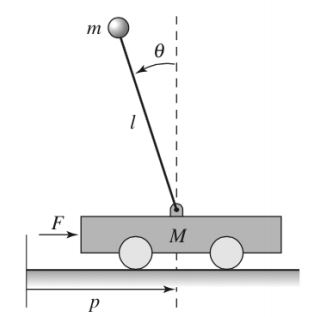
\includegraphics[width=0.8\textwidth]{mass_and_cart.jpg}
\caption{Inverted Pendulum on a cart diagram}
\end{figure}
\end{center}




The parameters of this system are:
\vspace{\baselineskip}

\vspace{\baselineskip} $\rightarrow$ the damping of the pendulum ($\rho$)

$\rightarrow$ the damping of the cart ($c$)

$\rightarrow$ the mass of the cart ($M$)

$\rightarrow$ the mass of the pendulum as a point load ($m$) at distance (%$l$)

$\rightarrow$ the acceleration sure to gravity ($g$)

$\rightarrow$ the position of the cart ($p$) and derivatives ($\dot{p}$, $\ddot{p}$)

$\rightarrow$ the angle of the pendulum ($th$) and derivatives ($\dot{\theta}$, $\ddot{\theta}$)

\vspace{\baselineskip}

Using Lagrange's equations, the equations of motion for this system can be expressed. 

The lagrangian ($L$) is kinetic energy taken away from potential energy, as such:


\vspace{\baselineskip} 
$L = T - V$
\vspace{\baselineskip}


for this system, the kinetic energy of the point mass ($m$) is made up of vertical and horizontal components, where the velocity in the horizontal will be decreased due to the linking cart's velocity. As such, the kinetic energy of the system is;


\vspace{\baselineskip}

$K = \frac{1}{2} m (\dot{p} - l \times \dot{\theta} cos(\theta))^2 + \frac{1}{2} m (l \times \dot{\theta} sin(\theta))^2 + \frac{1}{2} M \dot{p}^2$

\vspace{\baselineskip}


and the potential energy is contributed from the pendulum falling with increasing theta, such that;


\vspace{\baselineskip}

$V = m g l cos(\theta)$


\vspace{\baselineskip}


Langrange's equation states that:


\vspace{\baselineskip}


$\frac{d}{dt} (\frac{\partial L}{\partial q_d}) - \frac{\partial L}{\partial q} = Q$


\vspace{\baselineskip}


where Q is the non-conservative forces acting on the system, and $q$ is a coordinate system.


\vspace{\baselineskip}


Thus, for position, $p$;


\vspace{\baselineskip}


$\frac{d}{dt} (\frac{\partial L}{\partial \dot{p}}) - \frac{\partial L}{\partial p} = F - c \dot{p}$


\vspace{\baselineskip}


thus, where;


\vspace{\baselineskip}


$\frac{\partial L}{\partial \dot{p}} =  \frac{\partial}{\partial \dot{p}} (\frac{1}{2} m (\dot{p}^2 - 2 \dot{p} l \times \dot{\theta} cos(\theta) + l^2 \times \dot{\theta}^2 cos(\theta))) + M\dot{p}$


\vspace{\baselineskip}


$ = m(\dot{p} + l \times \dot{\theta} cos(\theta) + M \dot{p}$


\vspace{\baselineskip}
 
thus,


\vspace{\baselineskip}


$\frac{d}{dt} (\frac{\partial L}{\partial \dot{p}}) = m \ddot{p} - m l \times \ddot{\theta} cos(\theta) + m l \times \dot{\theta}^2 sin(\theta) + M \ddot{p} $


\vspace{\baselineskip}

and 

\vspace{\baselineskip}


$\frac{\partial L}{\partial p} = 0$


\vspace{\baselineskip}


thus the lagrangian about p is;


\vspace{\baselineskip}


$F - c \dot{p} = M \ddot{p} + m \ddot{p} - m l \times \ddot{\theta} cos(\theta) + m l \times \dot{\theta}^2 sin(\theta)$


\vspace{\baselineskip}
 

similarly for theta;


\vspace{\baselineskip}

$\frac{\partial L}{\partial \dot{\theta}} = \frac{1}{2} m \frac{\partial}{\partial \dot{\theta}} (\dot{p}^2 - 2 \dot{p} l \times \dot{\theta} cos(\theta) + l^2 \times \dot{\theta}^2 cos(\theta)^2 + l^2 \times \dot{\theta}^2 sin(\theta)^2)$


\vspace{\baselineskip}


$ = \frac{1}{2} m(-2 \dot{p} l cos(\theta) + 2 l^2 \times \dot{\theta} cos(\theta)^2 + 2 l^2 \times \dot{\theta} sin(\theta)^2)$


\vspace{\baselineskip}


$= -m \dot{p} l cos(\theta) + l^2 m \dot{\theta}$


\vspace{\baselineskip}


$\frac{d}{dt}(\frac{\partial L}{\partial \dot{\theta}}) = -m \ddot{p} l cos(\theta) + m \dot{p} \times \dot{\theta} l sin(\theta) + l^2 m \ddot{\theta}$


\vspace{\baselineskip}


and
\vspace{\baselineskip}


$\frac{\partial L}{\partial th} = \frac{1}{2} m \frac{\partial}{\partial th} ( \dot{p}^2 - 2 \dot{p} l \times \dot{\theta} cos(\theta) + l^2 \times \dot{\theta}^2 cos(\theta)^2 +  l^2 \times \dot{\theta}^2 sin(\theta)^2 + 2 g l cos(\theta))$


\vspace{\baselineskip}


$= \frac{1}{2} m (2 \dot{p} l \times \dot{\theta} sin(\theta) + 2 g l sin(\theta))$


\vspace{\baselineskip}


$= m l sin(\theta) \times \dot{\theta} p + g m l sin(\theta)$


\vspace{\baselineskip}


putting these together gives


\vspace{\baselineskip}


$\rightarrow -\rho \times \dot{\theta} = m l^2 \ddot{\theta} - m l \ddot{p} cos(\theta) + m l \dot{p} \times \dot{\theta} sin(\theta)  - m l sin(\theta) \times \dot{\theta} p - g m l sin(\theta)$


\vspace{\baselineskip}

thus the two equations of motion are:


\vspace{\baselineskip}


$ -\rho \times \dot{\theta} = m l^2 \times \ddot{\theta} - m l cos(\theta) \ddot{p} - m g l sin(\theta)$


\vspace{\baselineskip}



$F - c \dot{p} = (M+m) \ddot{p} + m l \times \dot{\theta}^2 sin(\theta) - m l \times \ddot{\theta} cos(\theta)$


\vspace{\baselineskip}



From here the state-space representation of the system can be obtained by small angle approximation, and rewriting the equations of motion in terms of $\frac{dx}{dt}$, where x is;


\vspace{\baselineskip}


$x_1 = p$, $x_2 = th$, $x_3 = \dot{p}$, and $x_4 = \dot{\theta}$


\vspace{\baselineskip}


which gives:


\vspace{\baselineskip}


$\frac{d x_1}{dt} = x_3$


\vspace{\baselineskip}


$\frac{d x_2}{dt} = x_4$


\vspace{\baselineskip}


$\frac{d x_3}{dt} = \frac{F}{M} - \frac{C}{M} x_3 + \frac{mg}{M} x_2 - \frac{\rho}{l\times M} x_4$


\vspace{\baselineskip}


$\frac{d x_4}{dt} = \frac{g}{l} x_2 + \frac{M}{M \times l} - \frac{c}{M \times l} x_3 + \frac{mg}{M \times l} x_2 - \frac{\rho (M+m)}{M\times l^2 \times m} x_4$


\vspace{\baselineskip}


These can now be written in state-space form. This result can also be computed using Matlab to compute the linearisation from the aforementioned equations of motion; by solving the Jacobian.


\vspace{\baselineskip}


\vspace{\baselineskip}

\lstinputlisting[caption={PBA3\_1.m}]{PBA3_1.m}

\vspace{\baselineskip}



The expression $F(x)$, such that $\dot{x} = F(x)$, including non-linearities is representing by $F\_x$ in the Matlab script above; calculated using the same method as above but without small angle approximation. This gives:

\vspace{\baselineskip}


$F(x) = \left(\begin{array}{c} x_{3}\\ x_{4}\\ -\frac{\mathrm{rho}\, x_{4}\, \cos\!\left(x_{2}\right) - F\, l + c\, l\, x_{3} + l^2\, m\, {x_{4}}^2\, \sin\!\left(x_{2}\right) - g\, l\, m\, \cos\!\left(x_{2}\right)\, \sin\!\left(x_{2}\right)}{l\, \left( - 1\, m\, {\cos\!\left(x_{2}\right)}^2 + M + m\right)}\\ -\frac{M\, \mathrm{\rho}\, x_{4} + m\, \mathrm{rho}\, x_{4} - F\, l\, m\, \cos\!\left(x_{2}\right) - g\, l\, m^2\, \sin\!\left(x_{2}\right) + l^2\, m^2\, {x_{4}}^2\, \cos\!\left(x_{2}\right)\, \sin\!\left(x_{2}\right) - M\, g\, l\, m\, \sin\!\left(x_{2}\right) + c\, l\, m\, x_{3}\, \cos\!\left(x_{2}\right)}{l^2\, m\, \left( - 1\, m\, {\cos\!\left(x_{2}\right)}^2 + M + m\right)} \end{array}\right)$


\vspace{\baselineskip}


From Taylor's series expansion, it is known that this function can be approximated about a point; using the Jacobian. This is outlined in the code, where the equilibrium point for this system is $x = [0 0 0 0]$, as this defines the position where the pendulum is held still in the vertical position, without movement of the cart. The Jacobian is computed with respect to x for the state's matrix A, and with respect to F for the input matrix B. This gives the following state-space equation:


\vspace{\baselineskip}


$
\left(\begin{array}{c} \dot{x_{1}}\\ \dot{x_{2}}\\ \dot{x_{3}}\\ \dot{x_{4}} \end{array}\right)
 = 
 \left(\begin{array}{cccc} 0 & 0 & 1 & 0\\ 0 & 0 & 0 & 1\\ 0 & \frac{g\, m}{M} & -\frac{c}{M} & -\frac{\mathrm{rho}}{M\, l}\\ 0 & \frac{g\, \left(M + m\right)}{M\, l} & -\frac{c}{M\, l} & -\frac{\mathrm{rho}\, \left(M + m\right)}{M\, l^2\, m} \end{array}\right)
\left(\begin{array}{c} x_{1}\\ x_{2}\\ x_{3}\\ x_{4} \end{array}\right)
+
\left(\begin{array}{c} 0\\ 0\\ \frac{1}{M}\\ \frac{1}{M\, l} \end{array}\right)
*F$


\vspace{\baselineskip}



It can be seen that this system of equations was the same as that derived from small angle approximation; shown above.

Substituting in parameter values: M = 10 kg,	 m = 80 kg,	
c = 0.1N/m/s,	 l = 1m,	rho = 0.01Nms,	 g = 9.81m/$s^2$

thus the state-space equation becomes:

\vspace{\baselineskip}


$
\left(\begin{array}{c} \dot{x_{1}}\\ \dot{x_{2}}\\ \dot{x_{3}}\\ \dot{x_{4}} \end{array}\right)
 = 
 \left(\begin{array}{cccc} 0 & 0 & 1.0 & 0\\ 0 & 0 & 0 & 1.0\\ 0 & 78.48 & -0.01 & -0.001\\ 0 & 88.29 & -0.01 & -0.001125 \end{array}\right)
\left(\begin{array}{c} x_{1}\\ x_{2}\\ x_{3}\\ x_{4} \end{array}\right)
+
\left(\begin{array}{c} 0\\ 0\\ 0.1\\ 0.1 \end{array}\right)
*F$


\vspace{\baselineskip}


All of the mathmatics for these steps is completed using Matlab, as outlined in the above snippet of code.

\clearpage

\section{Question 2}

To construct a Simulink model of the system, the equations of motion had to be written in such a way that $\dot{p}$ can be integrated to $p$, and $\dot{\theta}$ integrated to give $th$. This can be done by writing one equation in terms of $\ddot{\theta}$, and the other in terms of $\ddot{p}$, allowing integration to achieve the state variables ($p$, $th$, $\dot{p}$, $\dot{\theta}$). In doing this, the outputs end at the right hand side of the simulink model and the input force at the left.

\vspace{\baselineskip}


With the first equation of motion:


\vspace{\baselineskip}


$ -\rho \times \dot{\theta} = m l^2 \ddot{\theta} - m l cos(\theta) \ddot{p} - m g l sin(\theta)$


\vspace{\baselineskip}


$m l^2 \times \ddot{\theta} = m g l sin(\theta) + m l \ddot{p} cos(\theta) - \rho \dot{\theta}$


\vspace{\baselineskip}


$\therefore \ddot{\theta} = \frac{g}{l} sin(\theta) + \frac{\ddot{p}}{l} cos(\theta) - \frac{\rho}{m l^2} \times \dot{\theta}$


\vspace{\baselineskip}


similarly:


\vspace{\baselineskip}



$F - c \dot{p} = (M+m) \ddot{p} + m l \times \dot{\theta}^2 sin(\theta) - m l \times \ddot{\theta} cos(\theta)$


\vspace{\baselineskip}


substituting in the equation above (solve for $\ddot{\theta}$)


\vspace{\baselineskip}


$= (M + m) \ddot{p} + m l \dot{\theta}^2 sin(\theta) - ml cos(\theta) \frac{g}{l} sin(\theta) - m l cos(\theta) \frac{\ddot{p}}{l} cos(\theta) + m l cos(\theta) \frac{\rho}{m l^2} \times \dot{\theta}$


\vspace{\baselineskip}


$= (M + m -m cos(\theta)^2) \ddot{p} + m l \times \dot{\theta}^2 sin(\theta) - m g 
cos(\theta) sin(\theta) + \frac{\rho}{l} \dot{\theta} cos(\theta)$


\vspace{\baselineskip}


$\therefore \ddot{p} = \frac{1}{M + m -m cos(\theta)^2}  (F - c \dot{p} - m l \times \dot{\theta}^2 sin(\theta) + m g cos(\theta) sin(\theta) - \frac{\rho}{l} \dot{\theta} cos(\theta))$


\vspace{\baselineskip}


From this, the following simulink model was generated.


\vspace{\baselineskip}

\begin{center}
\begin{figure}[htb]
	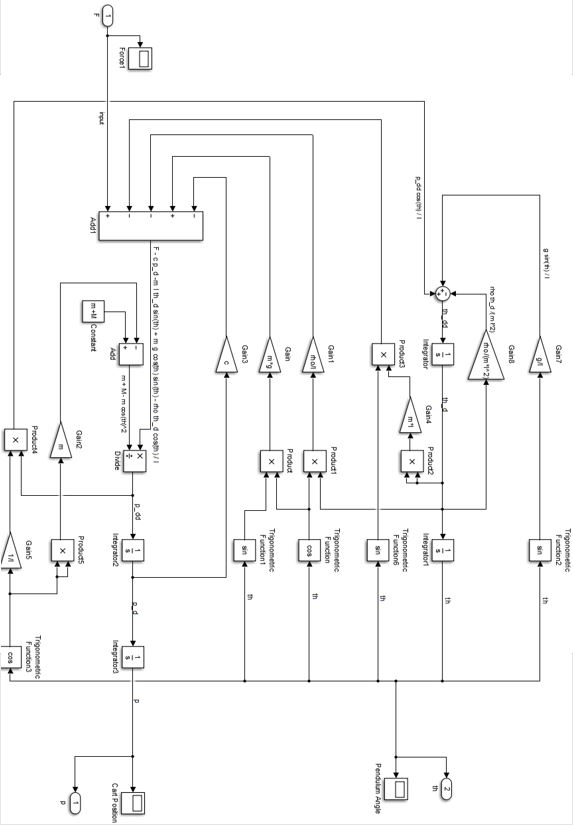
\includegraphics[width=1\textwidth]{PBA3_2_model_LS_3.jpg}
\caption{Simulink Model of Pendulum and Cart System}
\end{figure}
\end{center}


\clearpage


\section{Question 3}
The state-space representation of the simulink model made in question two can be computed using Matlab's linmod command; which requires an equilibrium point to be able to linearise the system. The script below displays the code required to do this task, and computes the eigenvalues of A to show that the it is the same model as the analysis in question 1.


\vspace{\baselineskip}

\lstinputlisting[caption={PBA3\_2\_script.m}]{PBA3_2_script.m}

\vspace{\baselineskip}

it can be seen that the equilibrium point was the same as that used in question 1, and the input to the system is 0.

In the script of question 1, the eigenvalues of A (represented by the variable EIG) were computed to be:


\vspace{\baselineskip}


$\lambda = \left(\begin{array}{c} 0\\ 9.3913\\ -9.4013\\ -0.0011 \end{array}\right)$


\vspace{\baselineskip}


this is transparent to the simulation as (the variable $EIG\_sim$):


\vspace{\baselineskip}


$\lambda = \left(\begin{array}{c} 0\\ -9.4013\\ 9.3913\\ -0.0011 \end{array}\right)$


\vspace{\baselineskip}


and thus they are the same.


\vspace{\baselineskip}


Similarly it can be seen that the state-space representation of the simulation is equivalent to that of question 1 (where $A = sys.a$, $B = sys.b$ in the previous code):


\vspace{\baselineskip}


$
\left(\begin{array}{c} \dot{x_{1}}\\ \dot{x_{2}}\\ \dot{x_{3}}\\ \dot{x_{4}} \end{array}\right)
 = 
 \left(\begin{array}{cccc} 0 & 0 & 1.0 & 0\\ 0 & 0 & 0 & 1.0\\ 0 & 78.48 & -0.01 & -0.001\\ 0 & 88.29 & -0.01 & -0.0011 \end{array}\right)
\left(\begin{array}{c} x_{1}\\ x_{2}\\ x_{3}\\ x_{4} \end{array}\right)
+
\left(\begin{array}{c} 0\\ 0\\ 0.1\\ 0.1 \end{array}\right)
*F$


\vspace{\baselineskip}



\section{Question 4}
Given the system is controllable, the poles of the system can be repositioned using state-feedback. The controllability of the system is determined by ensuring the controllability matrix has a determinant not equal to 0; implying the linear independence and invertibility.

The controllability matrix is;


\vspace{\baselineskip}


$ W = [ (B) (A B) (A^2 B) (A^3 B)]$


\vspace{\baselineskip}

Computing the determinant of this matrix can be done in Matlab; using the symbolic A 
and B from part 1. This gives;


\vspace{\baselineskip}


$det(W) = -\frac{g^2}{M^4\, l^4}$


\vspace{\baselineskip}


This is not equal to 0 so long as there is gravity, and doesn't exist if there is no cart mass or pendulum length. Thus, state-feedback can be used with the control law 


\vspace{\baselineskip}


$u = - K x $


\vspace{\baselineskip}


state feedback has the form:


\vspace{\baselineskip}


$\dot{x} = (A - K B) x$


\vspace{\baselineskip}


where is a 4x4 matrix which will change the poles of the system to those desired; stabilising the system.


\vspace{\baselineskip}


The feedback matrix K can be computed using Matlab's acker function, which takes in the state-space matrices of the system, and a matrix defining the desired pole locations.


\vspace{\baselineskip}


To stabilize the system, the poles must be placed in the left hand plane (the general expression is $y = exp(\lambda t)$, thus if $\lambda$ is negative the response of the system will decay to a steady state). The position of the poles will drastically affect the system's response, and thus must be chosen more wisely than just having 4 random negative poles. The closer the poles to the imaginary axis, the slower the response time, however the further the poles the more susceptible and responsive the system becomes to noise (high frequency). If the poles are positioned too far away from the imaginary axis, the desired response could be too quick for the actuator to perform (saturation). Therefore, it is important to decide poles on application, where in this case the system replicates that of a segway. A segway will be driven at the base, carrying a adult load (pendulum mass) and have a pendulum / handle length of a meter. In this application it would be important to have a fast response time such that hitting a small bum in the road wouldn't create a long duration, noticeable sway of. Additionally, it would be undesirable to have poles with a low damping ratio (perhaps anything smaller than 0.707) such that oscillation occurs; as the pendulum will sway back and forth with disturbances. In the s-place, this refers to complex conjugate poles with a higher imaginary component than that of it's negative real component.


\vspace{\baselineskip}


There are multiple different ways to simulate different disturbances to acknowledge how the chosen poles respond, and whether they need to be rethought; one can change the mass of the pendulum (to replicate the experience for a child instead of a 80kg person), add a disturbance acceleration to mimic a bump on the ground, or similarly add an impulse or step force to the base of the pendulum. 

The poles chosen for this section were


\vspace{\baselineskip}


$P = \left(\begin{array}{cccc} (-4+2i) & (-4-2i) & (-20+10i) & (-20-10i) \end{array}
\right)$


\vspace{\baselineskip}


this will produce a response with $\zeta = 0.8944$ and a dominant natural frequency of $4.472 rad/sec$; the poles were moved into this position by considering required gain of the system, where one maximum gain (of K) is 19477, which is assumed to be high in itself. It is believe that the second conjugate pair are fair enough from the dominant pair that they will have a minimal effect on the response, without drastically increasing the system's sensitivity to noise.


\vspace{\baselineskip}


Using the acker function, as seen in the below code, results in the following K matrix for the aforementioned pole placement.


\vspace{\baselineskip}


$K = \left(\begin{array}{cccc} -10193.68 & 19477.19 & -4893.19 & 5373.08 \end{array}\right)$


\vspace{\baselineskip}

\lstinputlisting[caption={PBA3\_4\_script.m}]{PBA3_4_script.m}

\vspace{\baselineskip}


Using the code towards the bottom of the above script, the step response of the system can be illustrated (however it uses the simulink model made in question 5 of this assignment, but it's response is useful to see how changing the poles can change the response of this system):
\vspace{\baselineskip}

\begin{center}
\begin{figure}[htb]
	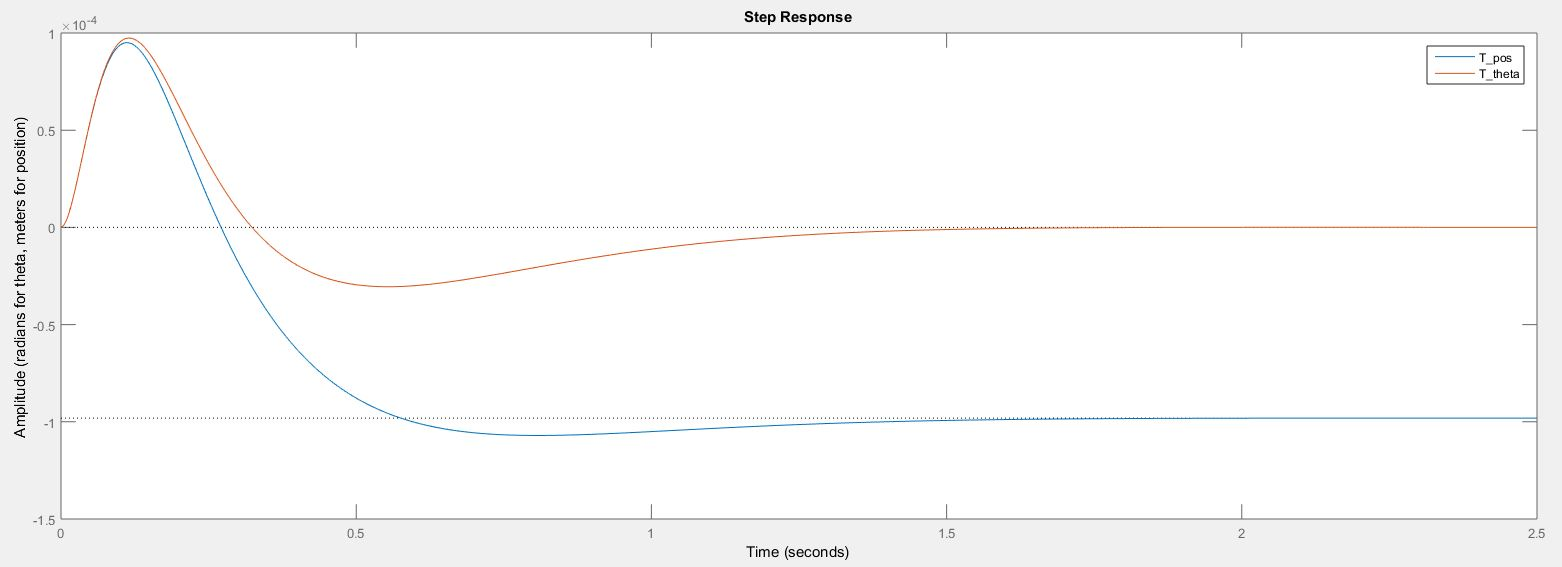
\includegraphics[width=1\textwidth]{PBA3_time_response.jpg}
\caption{Step response of pendulum angle and cart position}
\end{figure}
\end{center}



\clearpage


\section{Question 5}
The model made in question 2 is illustrated below with state feedback; each state is multiplied by it's corresponding gain from the matrix K and fed in as input to the system such that $u = -K x$. This is illustrated on the following page; a bit cramped to fit the width on the page, but the key difference is the four gain stages at the bottom of the model.





\begin{center}
\begin{figure}[htb]
	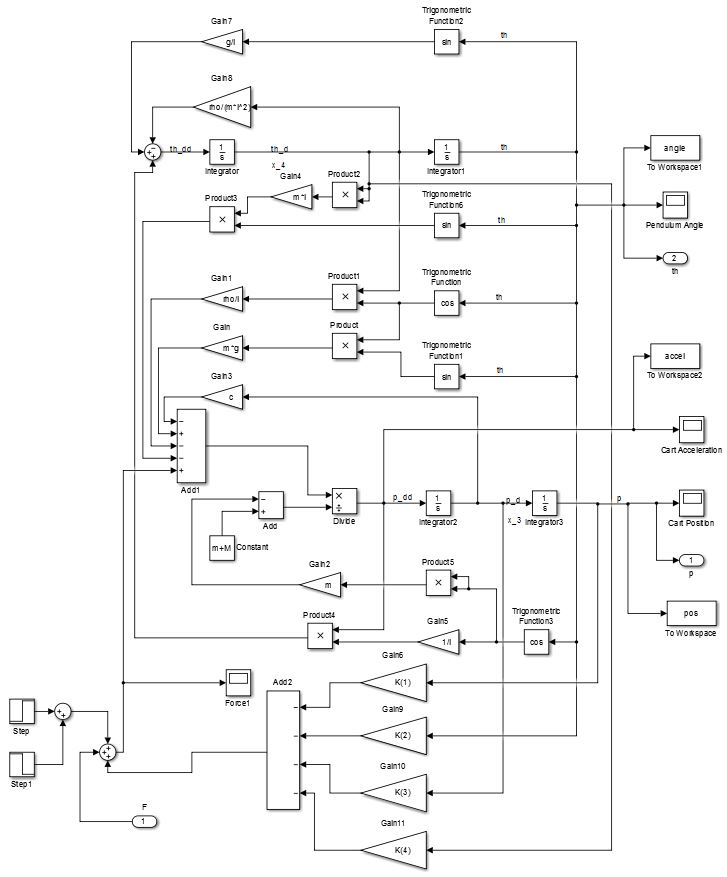
\includegraphics[width=1.1\textwidth]{PBA3_5_model.jpg}
\caption{Simulink Model of Pendulum and Cart System with state feedback}
\end{figure}
\end{center}

\clearpage

\begin{center}
\begin{figure}[htb]
	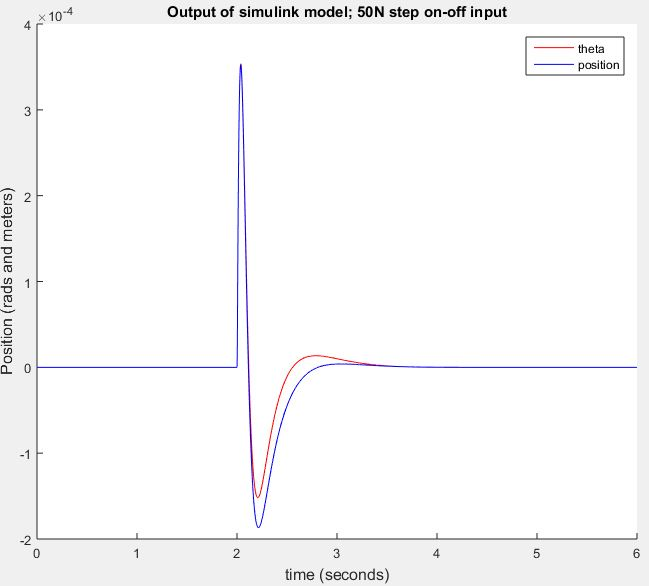
\includegraphics[width=0.9\textwidth]{PBA3_5_50N_response.jpg}
\caption{Response of 50N step on-off force applied to state feedback system at input}
\end{figure}
\end{center}

It was found that this system is very robust to disturbances(having started at equilibrium), where a 200N impulse and a ramp disturbance on theta with a slope of 2, and changing the length and mass of the pendulum wasn't able to considerably move the pendulum angle, or make unstable; mainly due to the high frequency poles. If however, the initial state of theta was $\pi /2$ it was found that the system became unstable; thus the system is locally asymptotically stable, as a change in initial conditions has rendered the system unstable. In addition to this, if the poles of this system were moved closer to the imaginary axis, they responded slower to system disturbances, thus it was found that poles with real components -1, -1, -2, -2, led to an unstable system when a 70N force was applied at the input for 1 second. These are both illustrated below.

\begin{center}
\begin{figure}[htb]
	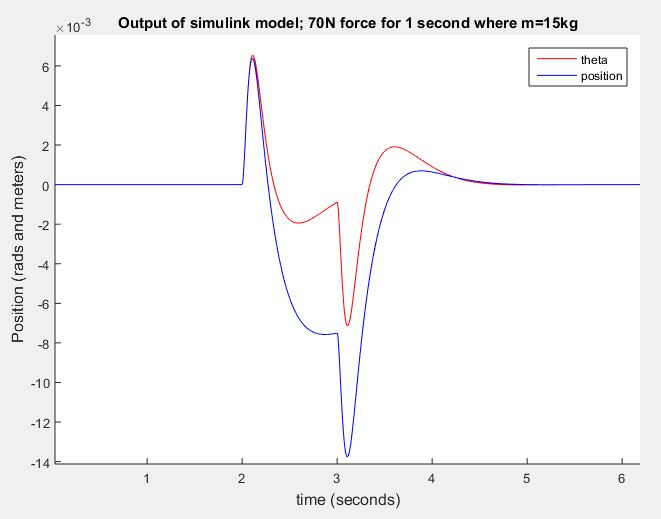
\includegraphics[width=0.9\textwidth]{PBA3_5_m_15.jpg}
\caption{Response of 70N step on-off 1 sec force, where m=15kg, it can be seen that a greater amplitude of oscillation occurred, however it is unrecognisable for the rider}
\end{figure}
\end{center}


\begin{center}
\begin{figure}[htb]
	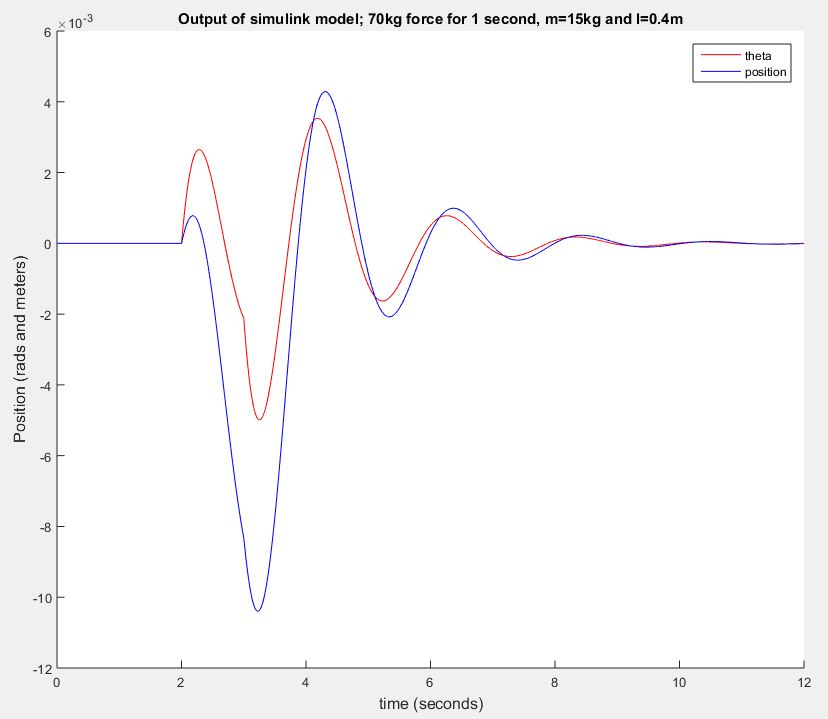
\includegraphics[width=0.9\textwidth]{PBA3_5_m15_l40.jpg}
\caption{Response of 70N step on-off 1 sec force, where m=15kg and l=0.4m, it can be seen that a greater amplitude of and more oscillation occurred, however it is unrecognisable for the rider}
\end{figure}
\end{center}


\begin{center}
\begin{figure}[htb]
	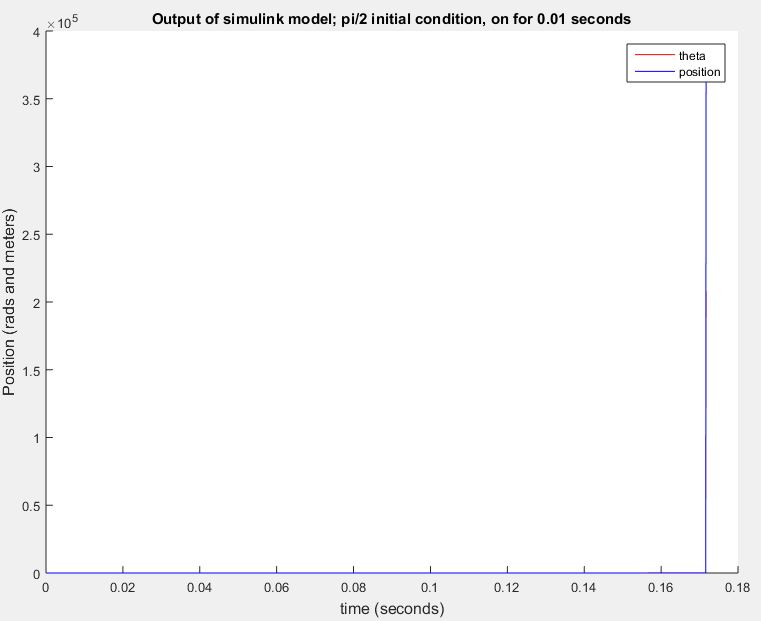
\includegraphics[width=0.9\textwidth]{PBA3_5_th_dist.jpg}
\caption{Response of 70N step on-off 1 sec force, with 0.01 second initial step added to theta}
\end{figure}
\end{center}



\begin{center}
\begin{figure}[htb]
	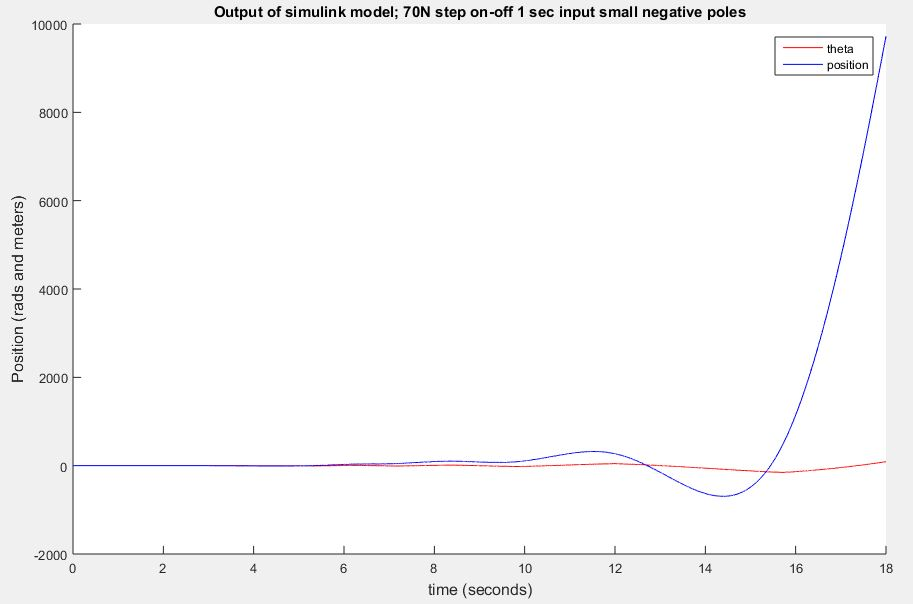
\includegraphics[width=0.9\textwidth]{PBA3_5_70N_response2.jpg}
\caption{Response of 70N step on-off 1 sec force applied to state feedback system at input for poles at -1, -1, -2, -2}
\end{figure}
\end{center}




\clearpage

\end{document}